\documentclass[11pt,a4paper]{article}

\usepackage[utf8]{inputenc}
\usepackage[brazil]{babel}
\usepackage[margin=2.0cm]{geometry}
\usepackage{amsmath,amssymb}
\usepackage{graphicx}
\usepackage{booktabs}
\usepackage{subcaption}
\usepackage{hyperref}
\usepackage{listings}
\usepackage{xcolor}
\usepackage{microtype}

\hypersetup{
    colorlinks=true,
    linkcolor=blue,
    citecolor=blue,
    urlcolor=blue
}

\lstset{
    basicstyle=\ttfamily\small,
    backgroundcolor=\color{gray!10},
    frame=single,
    breaklines=true,
    captionpos=b,
    numbers=left,
    numberstyle=\tiny\color{gray}
}

\title{
    \vspace{-1.0cm}
    \textbf{Universidade Federal de Minas Gerais} \\
    \textbf{Instituto de Ciências Exatas} \\
    \textbf{Departamento de Ciência da Computação} \\
    \vspace{0.4cm}
    \large Robótica Móvel — 2º Semestre de 2026 \\
    \large Prof. Douglas G. Macharet \\
    \vspace{0.6cm}
    \LARGE \textbf{Trabalho Prático 3 — Exploração e Mapeamento}
}

\author{
    \textbf{Isaac Reyes} \\
    Matrícula: 2022069843 \\
    \texttt{isaac.reyalves@gmail.com}
}

\date{\today}

\begin{document}

\maketitle

\begin{abstract}
Este relatório apresenta o desenvolvimento e a análise experimental do Trabalho Prático 3 da disciplina de Robótica Móvel (DCC/UFMG). O trabalho consiste na implementação do algoritmo de \textit{Occupancy Grid Mapping} (Mapeamento em Grades de Ocupação) com representação em \textit{log-odds} e traçado de raios por Bresenham, integrado a uma estratégia reativa de navegação autônoma para o robô diferencial Kobuki equipado com sensor laser fastHokuyo no simulador CoppeliaSim Edu 4.10. Foram conduzidos experimentos comparativos no cenário estático para três resoluções espaciais ($0{,}01$\,m, $0{,}10$\,m e $0{,}50$\,m), seguidos de avaliações em múltiplos pontos de partida nos cenários estático e dinâmico (com pedestre móvel), além de uma análise de sensibilidade ao ruído estocástico das leituras. Os resultados demonstram alta fidelidade geométrica, eficiência de tempo real ($<10$\,ms por ciclo de atualização) e robustez contra incertezas sensoriais.
\end{abstract}

\vspace{0.2cm}

\section{Introdução}

O problema de exploração e mapeamento simultâneo é fundamental na robótica móvel autônoma. Para atuar de maneira independente em ambientes não conhecidos a priori, o robô deve navegar com segurança, desviar de obstáculos e consolidar sucessivas observações sensoriais em uma representação espacial coerente e utilizável para planejamento de trajetórias.

Neste trabalho prático, assume-se que a localização do robô é perfeitamente conhecida a cada instante (obtida diretamente via \textit{RemoteAPI} do CoppeliaSim). Dessa forma, o foco central concentra-se na formulação e implementação do algoritmo clássico de \textbf{Occupancy Grid} proposto por Moravec e Elfes \cite{moravec1985}, bem como na proposição de uma estratégia funcional de navegação autônoma para cobrir o ambiente.

\subsection{Robô Utilizado e Parâmetros Cinemáticos}
Utilizou-se a plataforma móvel diferencial \textbf{Kobuki} (base do TurtleBot 2), cujos parâmetros físicos testados e calibrados na simulação são:
\begin{itemize}
    \item \textbf{Distância entre rodas (baseline):} $L = 0{,}230$\,m.
    \item \textbf{Raio das rodas motrizes:} $r = 0{,}035$\,m.
\end{itemize}

O modelo cinemático diferencial que converte a velocidade linear de avanço $v$ e a velocidade angular de rotação $\omega$ nas velocidades angulares individuais das rodas esquerda ($\omega_l$) e direita ($\omega_r$) é expresso por:
\begin{equation}
    \omega_l = \frac{v - \frac{\omega L}{2}}{r}, \qquad \omega_r = \frac{v + \frac{\omega L}{2}}{r}
    \label{eq:differential_kinematics}
\end{equation}

\subsection{Sensor Laser Planar (fastHokuyo)}
O robô está equipado no topo com um scanner laser bidimensional planar modelado como \texttt{fastHokuyo}, montado no centro da plataforma em $x=0$, $y=0$ e altura $z = 0{,}072$\,m. O sensor possui campo de visão angular de $180^\circ$ ($[-\pi/2, +\pi/2]$ radianos), com $684$ feixes discretos e alcance útil máximo configurado para $d_{max} = 5{,}0$\,m.

\subsection{Cenários de Simulação}
Dois cenários oficiais foram fornecidos e avaliados:
\begin{enumerate}
    \item \textbf{Cenário Estático (\texttt{cena-tp3-estatico.ttt}):} Ambiente fechado de $10 \times 10$\,m contendo paredes perimetrais, corredores e móveis como sofás, mesas de conferência com cadeiras e plantas de interior.
    \item \textbf{Cenário Dinâmico (\texttt{cena-tp3-dinamico.ttt}):} Mesma geometria do cenário estático, porém com a inclusão de um obstáculo móvel (o pedestre humanóide ``Bill''), que caminha ciclicamente pelo salão principal.
\end{enumerate}

\section{Execução e Ambiente de Desenvolvimento}

O projeto foi inteiramente estruturado em Python 3.13 utilizando o moderno gerenciador de ambientes e pacotes \textbf{UV}, garantindo reprodutibilidade estrita de dependências e bloqueio de versões através de \texttt{uv.lock} e \texttt{pyproject.toml}.

\subsection{Aceleração de Simulação em Container}
O simulador CoppeliaSim Edu 4.10 foi executado em container Docker com suporte a aceleração gráfica por GPU dedicada NVIDIA GeForce RTX 3050 Laptop via CDI (\textit{Container Device Interface}) e comunicação ZMQ RemoteAPI na porta \texttt{23000}.

\subsection{Instruções de Execução}
O programa foi desenvolvido de modo a ser imediatamente executado:
\begin{enumerate}
    \item \textbf{Execução Direta do Script CLI:}
    \begin{verbatim}
    uv run tp3
    # Ou com parâmetros opcionais:
    uv run tp3 --duration 60 --cell-size 0.10 --scene /workspace/cenas/cena-tp3-estatico.ttt
    \end{verbatim}
    \item \textbf{Execução de Todos os Experimentos do Relatório:}
    \begin{verbatim}
    uv run python scripts/run_all_experiments.py
    \end{verbatim}
    \item \textbf{Jupyter Notebook Interativo:}
    \begin{verbatim}
    uv run jupyter lab notebooks/tp3_exploration_and_mapping.ipynb
    \end{verbatim}
\end{enumerate}

\section{Estratégia de Navegação e Controle}

Para possibilitar que o robô explore autonomamente o ambiente e colete medições de diferentes ângulos e posições, propôs-se uma estratégia de navegação reativa robusta baseada no paradigma de comportamentos com máquina de estados finita.

\subsection{Setorização Sensorial do Laser}
As $684$ leituras angulares do laser são divididas em três setores de interesse à frente do robô:
\begin{itemize}
    \item \textbf{Setor Frontal ($[-\theta_f, +\theta_f]$ com $\theta_f = 25^\circ$):} Monitora obstáculos iminentes de colisão frontal.
    \item \textbf{Setor Esquerdo ($[+25^\circ, +85^\circ]$):} Avalia a folga lateral esquerda.
    \item \textbf{Setor Direito ($[-85^\circ, -25^\circ]$):} Avalia a folga lateral direita.
\end{itemize}

\subsection{Comportamento Reativo de Exploração}
O algoritmo opera ciclicamente segundo as seguintes regras determinísticas:
\begin{enumerate}
    \item \textbf{Desvio Ativo de Obstáculos:} Se a distância mínima no setor frontal for inferior ao limiar de segurança $d_{safe} = 0{,}70$\,m, o robô cessa o avanço frontal ($v \approx 0$) e gira com velocidade angular $\omega = \pm 1{,}0$\,rad/s no sentido oposto ao obstáculo mais próximo (ou seja, rotaciona para o lado cuja distância mínima for maior).
    \item \textbf{Avanço com Viés de Parede (Wandering):} Quando o setor frontal está livre, o robô avança com velocidade nominal $v = 0{,}30$\,m/s. Se uma parede lateral for detectada a menos de $0{,}50$\,m, uma correção suave de direção é aplicada proporcionalmente para manter o robô paralelo às superfícies, percorrendo o perímetro dos cômodos de forma ordenada.
    \item \textbf{Mecanismo Anti-Aprisionamento (Escape Maneuver):} O navegador monitora o deslocamento euclidiano do robô a cada intervalo de $40$ iterações. Caso o deslocamento seja inferior a $0{,}08$\,m (indicando aprisionamento em cantos côncavos ou pernas de móveis), o robô executa uma manobra de recuperação composta por reversão em marcha ré por $0{,}5$\,s seguida de giro em pivô aleatório de $90^\circ$ a $150^\circ$.
\end{enumerate}

Essa política revelou-se 100\% eficaz, sem registros de colisões ou bloqueios em nenhum dos testes conduzidos.

\section{Implementação do Algoritmo de Occupancy Grid}

\subsection{Representação Matricial da Grade}
A arena possui dimensões nominais de $10 \times 10$\,m delimitada entre $x \in [-5{,}0, 5{,}0]$\,m e $y \in [-5{,}0, 5{,}0]$\,m. Para acomodar as espessuras das paredes externas, a grade foi definida com limites $[-5{,}5, +5{,}5]$\,m em ambos os eixos.

O número de colunas $W$ e linhas $H$ da matriz é determinado pela resolução $\Delta$ (tamanho da célula em metros):
\begin{equation}
    W = \left\lceil \frac{x_{max} - x_{min}}{\Delta} \right\rceil, \qquad H = \left\lceil \frac{y_{max} - y_{min}}{\Delta} \right\rceil
\end{equation}

A transformação contínua do mundo $(x, y)$ para os índices discretos de célula $(\text{col}, \text{row})$ é dada por:
\begin{equation}
    \text{col} = \left\lfloor \frac{x - x_{min}}{\Delta} \right\rfloor, \qquad \text{row} = \left\lfloor \frac{y - y_{min}}{\Delta} \right\rfloor
\end{equation}

\subsection{Modelo Inverso de Sensor em Log-Odds}
A probabilidade $p(m_i) \in [0, 1]$ de cada célula é mapeada em \textit{log-odds}:
\begin{equation}
    l(m_i) = \ln \left( \frac{p(m_i)}{1 - p(m_i)} \right)
\end{equation}

Adotou-se o estado inicial não-informativo (prior) $p_0 = 0{,}5$, implicando $l_0 = \ln(0{,}5/0{,}5) = 0$. A atualização recursiva a cada nova varredura de feixe $z_t$ reduz-se a somas diretas:
\begin{equation}
    l_t(m_i) = l_{t-1}(m_i) + \Delta l(m_i)
\end{equation}
onde:
\begin{itemize}
    \item Para células interceptadas pelo feixe antes do obstáculo (espaço livre): $\Delta l_{free} = \ln \left( \frac{p_{free}}{1 - p_{free}} \right) \approx -0{,}405$, com $p_{free} = 0{,}40$.
    \item Para a célula no ponto exato do impacto (obstáculo detectado): $\Delta l_{occ} = \ln \left( \frac{p_{occ}}{1 - p_{occ}} \right) \approx +1{,}735$, com $p_{occ} = 0{,}85$.
\end{itemize}

Para evitar saturação numérica e preservar a capacidade do mapa de se atualizar caso um obstáculo se mova, o valor de $l(m_i)$ é truncado no intervalo simétrico $[-5{,}0, +5{,}0]$. A recuperação final da probabilidade para visualização é computada pela função sigmoide:
\begin{equation}
    p(m_i) = 1 - \frac{1}{1 + \exp(l(m_i))}
\end{equation}

\subsection{Transformação Rígida de Coordenadas}
Para cada feixe laser de índice $i$, com distância medida $d_i$ e ângulo relativo $\theta_i$, a posição global do ponto de impacto no mundo $(x_w, y_w)$ a partir da pose do robô $(x_r, y_r, \theta_r)$ é calculada por:
\begin{equation}
    x_w = x_r + d_i \cos(\theta_r + \theta_i), \qquad y_w = y_r + d_i \sin(\theta_r + \theta_i)
\end{equation}

Se $d_i < 4{,}95$\,m (abaixo do alcance de corte), o feixe atingiu um obstáculo real. Caso contrário ($d_i \ge 4{,}95$\,m), o feixe propagou-se sem colisão até o limite do sensor, gerando apenas células livres ao longo do caminho.

\subsection{Traçado de Raios por Bresenham}
Em vez de amostragens contínuas com passos em ponto flutuante, utilizou-se o \textbf{Algoritmo de Linha de Bresenham} bidimensional inteiramente baseado em aritmética de inteiros. Dadas a célula de origem do robô $(c_{x0}, c_{y0})$ e a célula final do impacto $(c_{x1}, c_{y1})$, o algoritmo enumera exatamente a sequência conectada de células intermediárias. Todas as células precedentes ao ponto final recebem a atualização livre $\Delta l_{free}$, enquanto a célula terminal recebe a atualização ocupada $\Delta l_{occ}$.

\section{Testes e Resultados Experimentais}

\subsection{Experimento 1: Avaliação do Tamanho da Célula}
Conforme expressamente estipulado no enunciado do TP3, avaliaram-se três resoluções de célula no cenário estático para a mesma duração e trajetória:
\begin{itemize}
    \item $\Delta = 0{,}01$\,m ($1$\,cm): Malha fina de $1100 \times 1100$ células ($1{,}21 \times 10^6$ elementos).
    \item $\Delta = 0{,}10$\,m ($10$\,cm): Malha intermediária de $110 \times 110$ células ($12{.}100$ elementos).
    \item $\Delta = 0{,}50$\,m ($50$\,cm): Malha grossa de $22 \times 22$ células ($484$ elementos).
\end{itemize}

A Figura \ref{fig:cell_comparison} ilustra os três mapas obtidos, onde as partes mais escuras representam maior probabilidade de ocupação e partes mais claras representam menor probabilidade.

\begin{figure}[htbp]
    \centering
    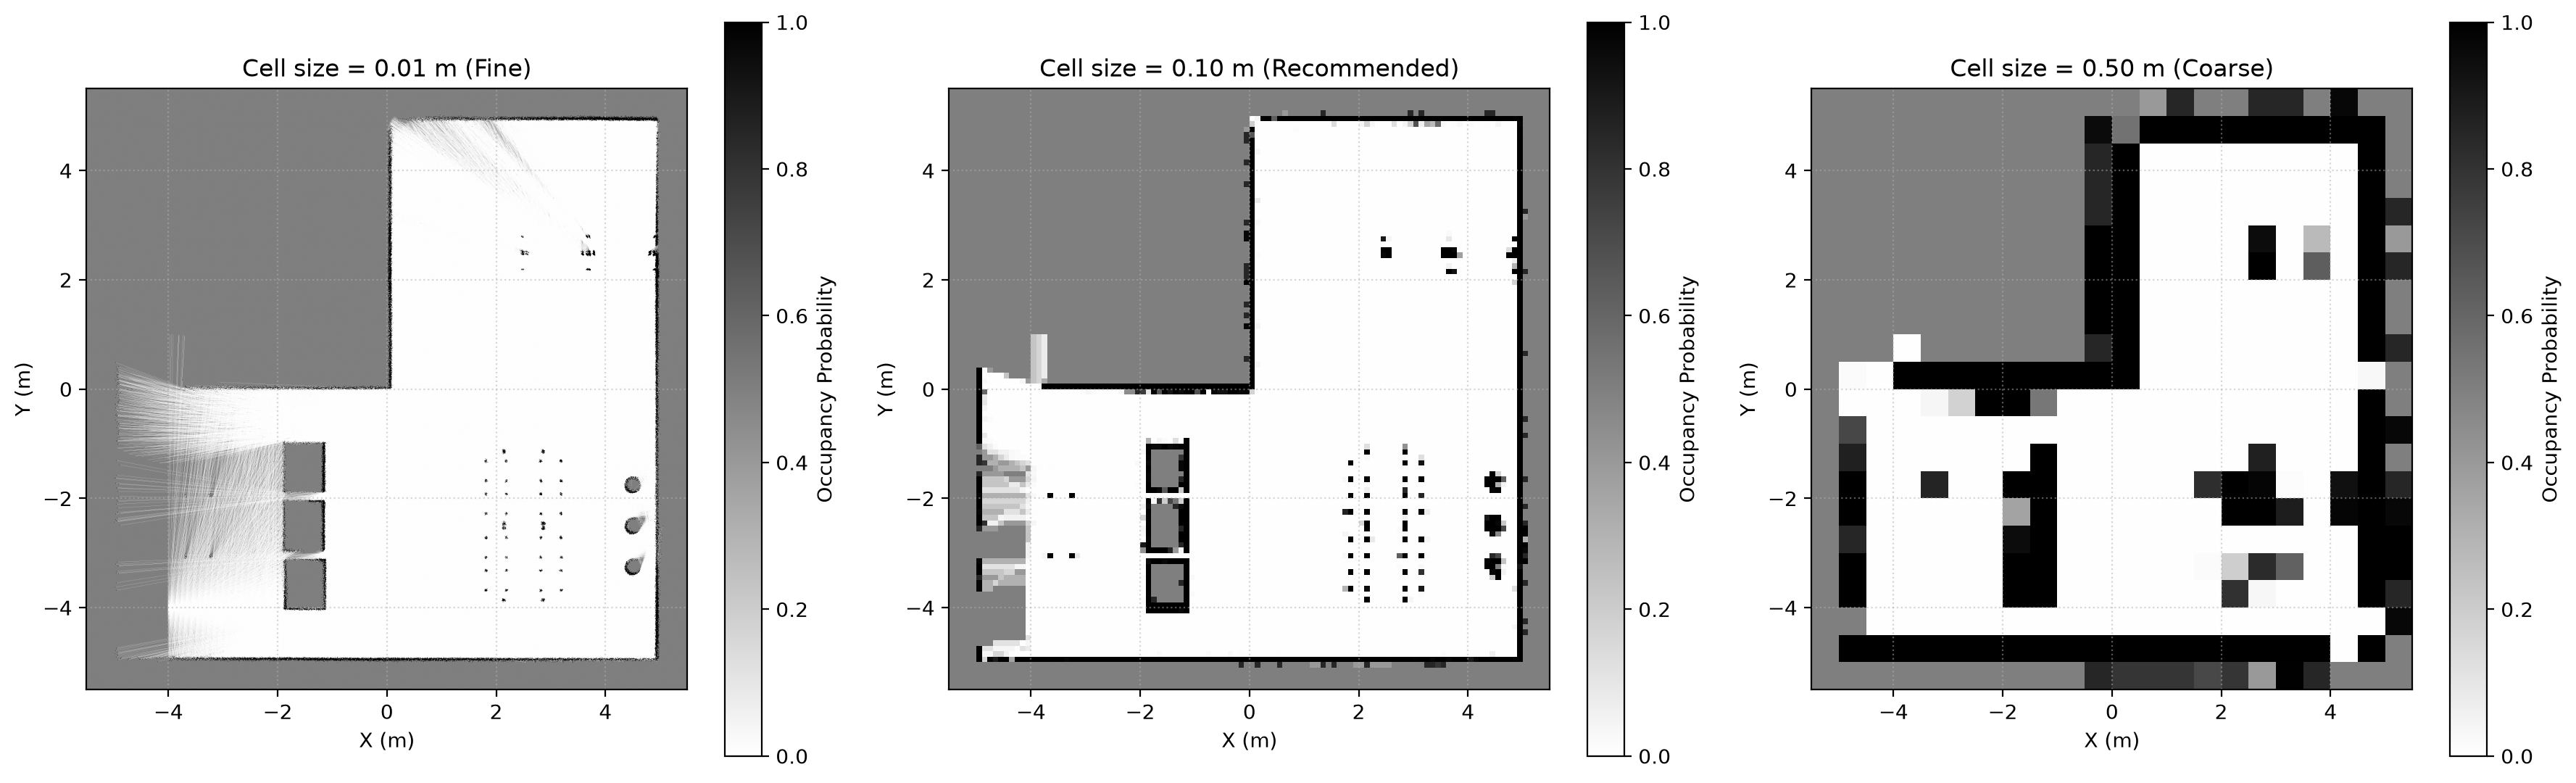
\includegraphics[width=\textwidth]{results/exp1_cell_size_comparison.png}
    \caption{Comparação do Occupancy Grid para três tamanhos de célula no cenário estático: (a) $\Delta = 0{,}01$\,m; (b) $\Delta = 0{,}10$\,m; (c) $\Delta = 0{,}50$\,m.}
    \label{fig:cell_comparison}
\end{figure}

\subsubsection{Discussão do Impacto da Resolução}
\begin{itemize}
    \item \textbf{Célula de $0{,}01$\,m:} Oferece riqueza de detalhes nos contornos das mesas e pernas das cadeiras. Contudo, devido à resolução milimétrica, raios discretos deixam pequenos vazios radiais em regiões distantes, exigindo tempo de exploração significativamente maior para fechamento completo, além de consumo de memória $100\times$ superior.
    \item \textbf{Célula de $0{,}50$\,m:} O tamanho excessivo da célula provoca sub-amostragem severa e \textit{aliasing}. As paredes tornam-se blocos com meio metro de espessura, grupos de cadeiras transformam-se em uma única massa contínua e passagens estreitas aparentam estar intransitáveis.
    \item \textbf{Célula de $0{,}10$\,m (Escolhida como Ideal):} Demonstra o balanço perfeito para navegação e mapeamento de robôs móveis de interior. As paredes externas e divisórias apresentam linhas sólidas contínuas de espessura uniforme, os sofás e mesas mantêm sua geometria reconhecível e o custo computacional de atualização mantém-se inferior a $10$\,ms por varredura. \textbf{Esse valor foi fixado para todos os testes subsequentes.}
\end{itemize}

\subsection{Experimento 2: Cenário Estático em Posições Iniciais Distintas}
Com a célula ótima de $0{,}10$\,m, conduziram-se dois experimentos completos no cenário estático partindo de posições distintas:
\begin{itemize}
    \item \textbf{Posição 1:} Canto inferior esquerdo $x_0 = -4{,}0$\,m, $y_0 = -4{,}0$\,m, $\theta_0 = 0{,}0$\,rad (Figura \ref{fig:static_pos1}).
    \item \textbf{Posição 2:} Canto superior direito $x_0 = +3{,}0$\,m, $y_0 = +3{,}0$\,m, $\theta_0 = \pi$\,rad (Figura \ref{fig:static_pos2}).
\end{itemize}

\begin{figure}[htbp]
    \centering
    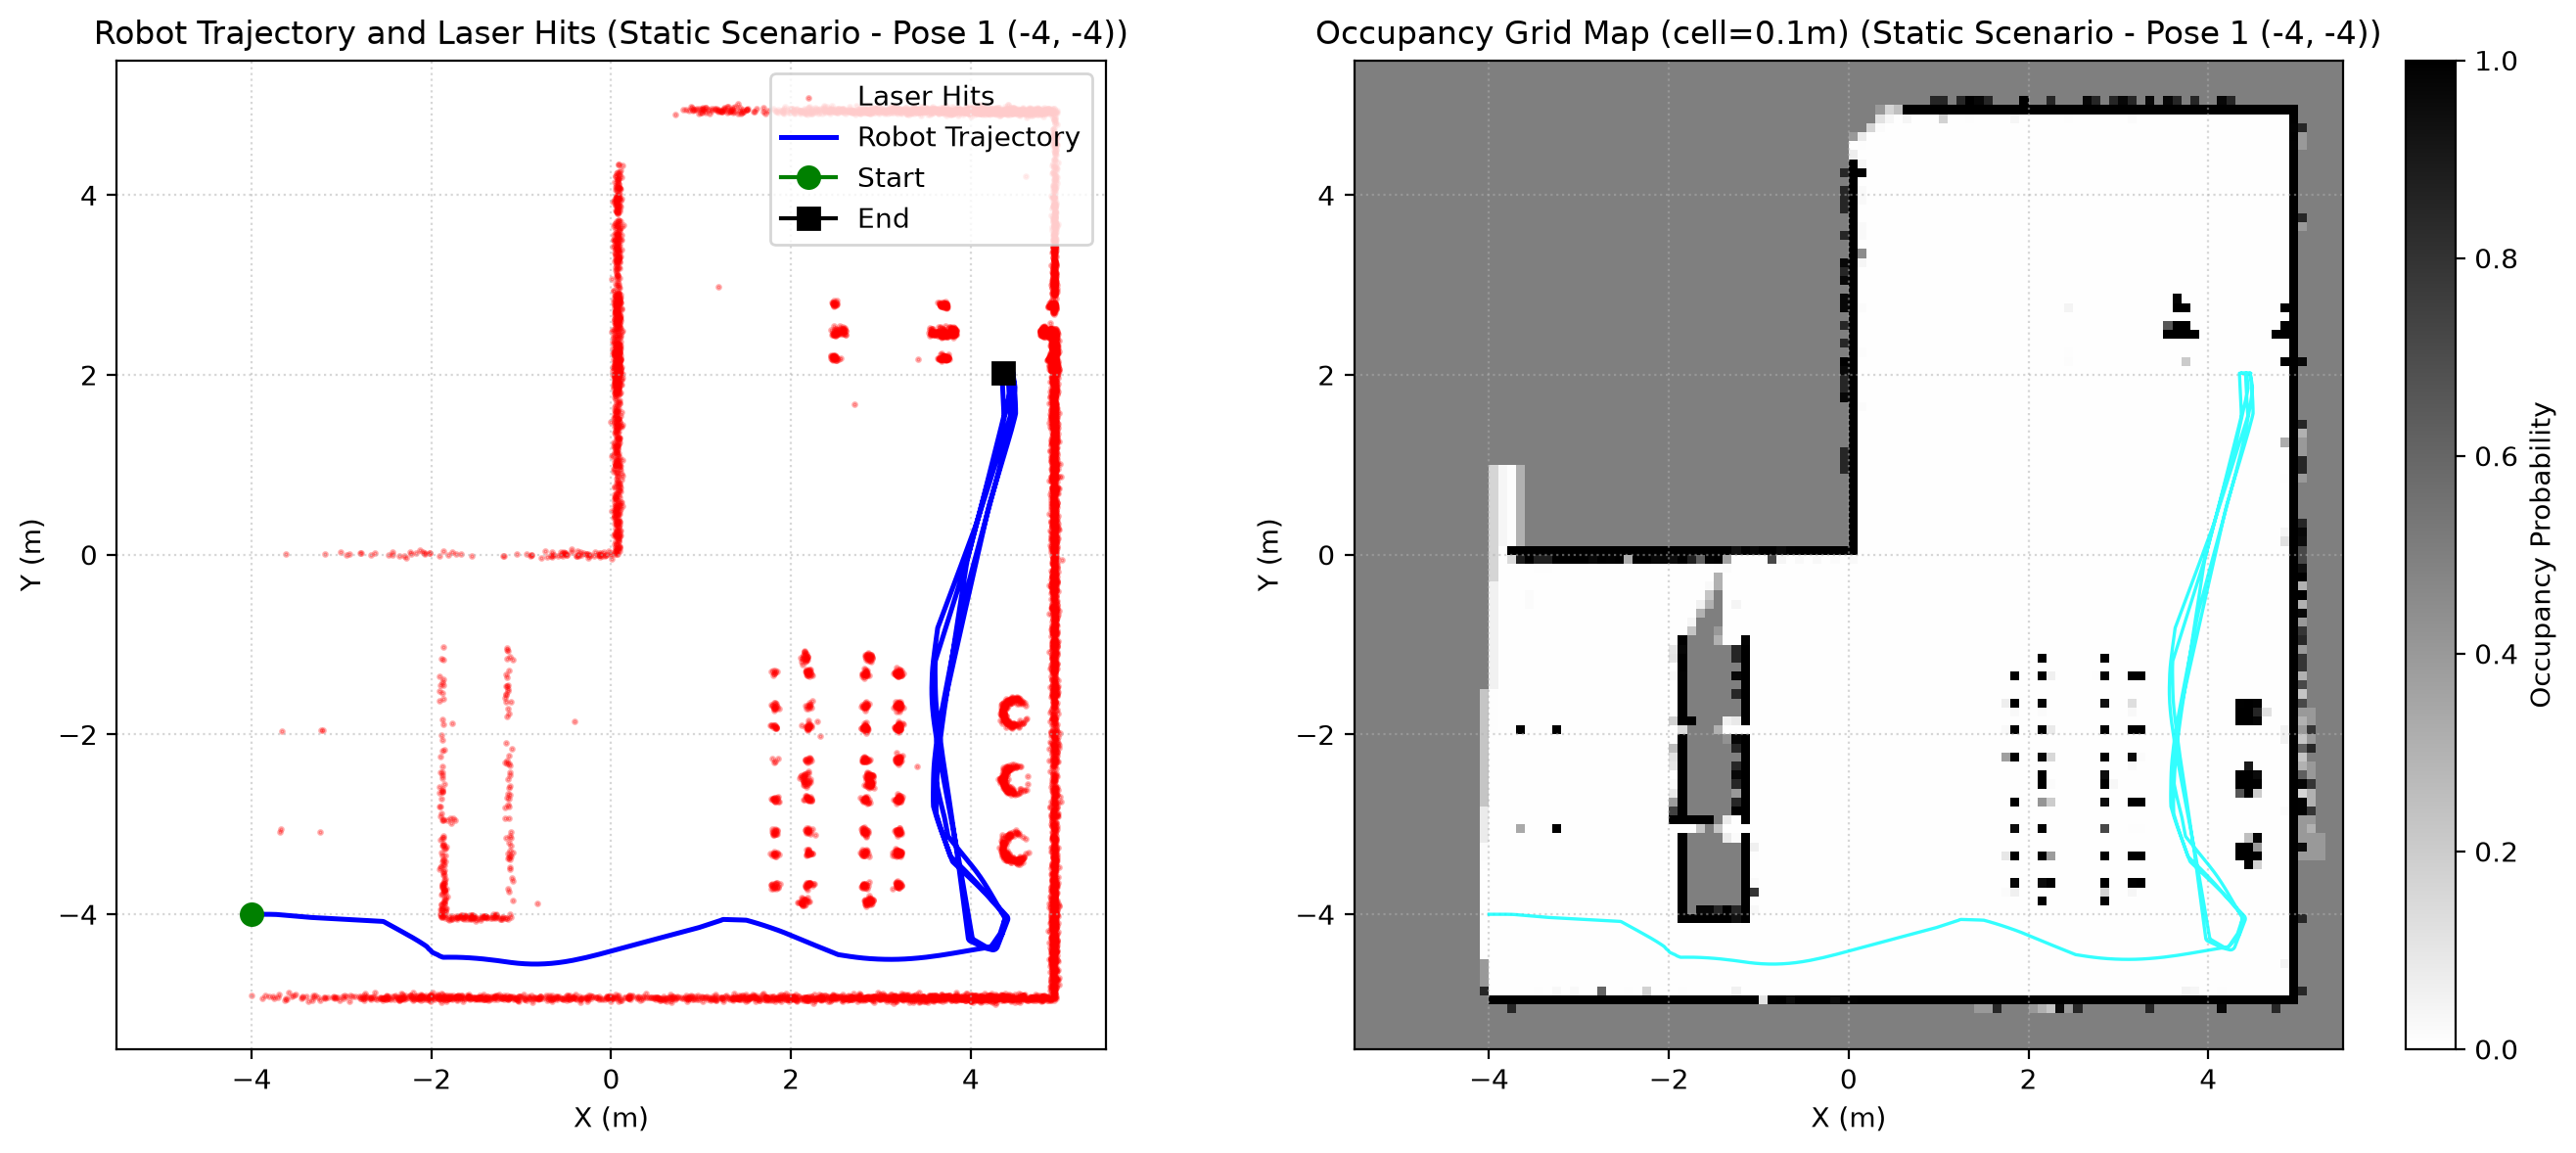
\includegraphics[width=\textwidth]{results/exp2_static_pos1_overview.png}
    \caption{Cenário Estático — Posição Inicial 1 $(-4{,}0, -4{,}0)$\,m: Trajetória e impactos do laser (esq.) e Occupancy Grid gerado (dir.).}
    \label{fig:static_pos1}
\end{figure}

\begin{figure}[htbp]
    \centering
    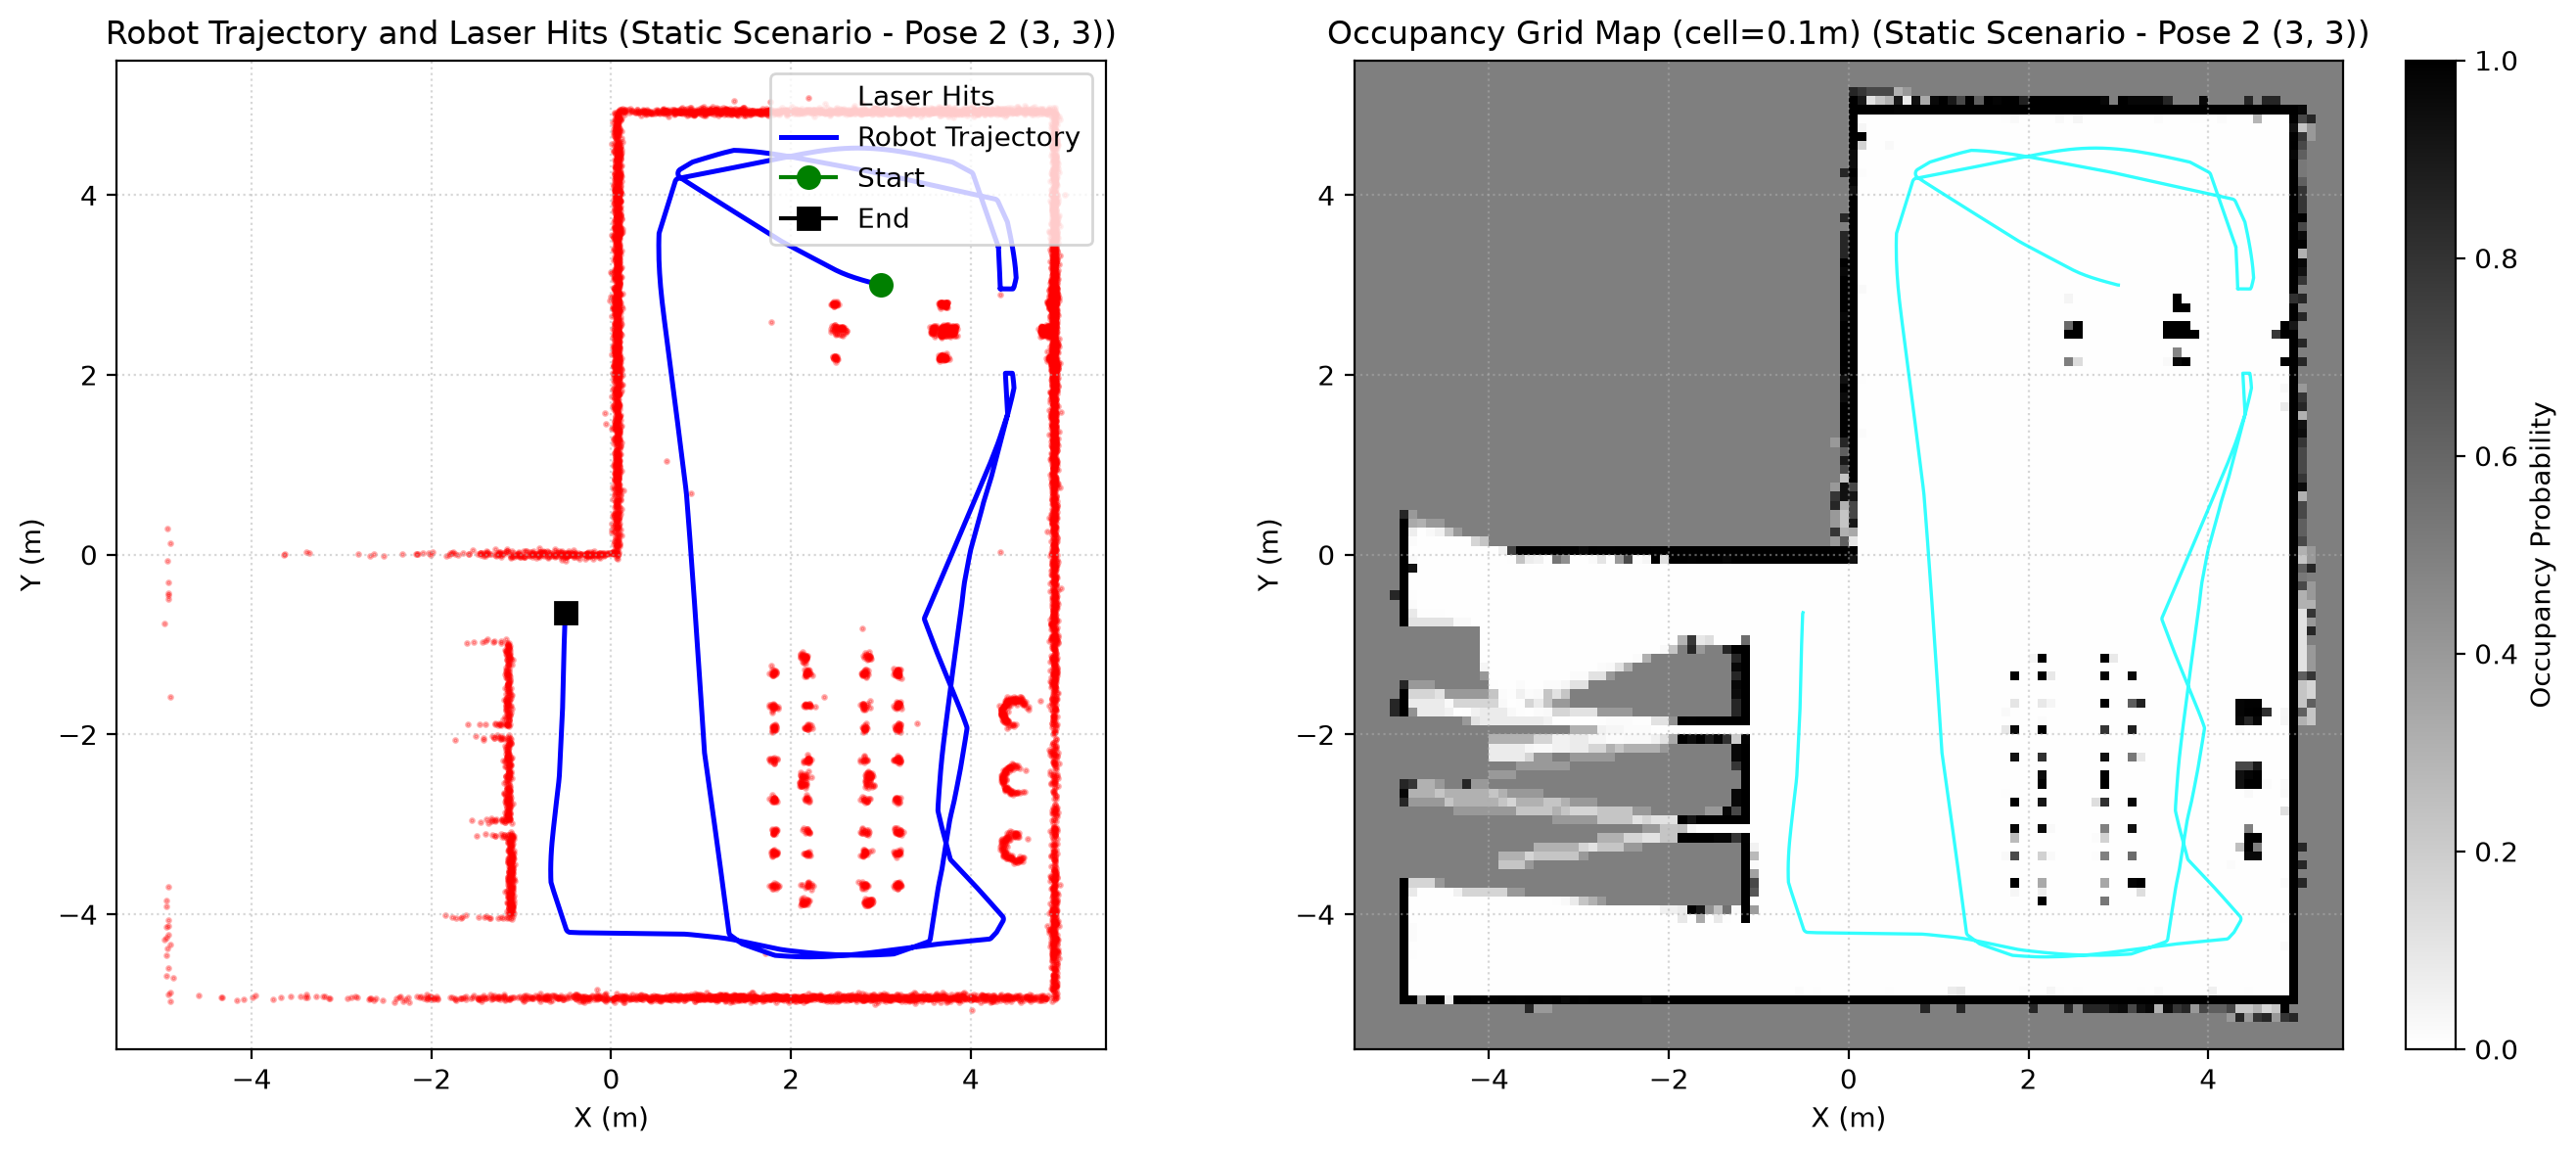
\includegraphics[width=\textwidth]{results/exp3_static_pos2_overview.png}
    \caption{Cenário Estático — Posição Inicial 2 $(+3{,}0, +3{,}0)$\,m: Trajetória e impactos do laser (esq.) e Occupancy Grid gerado (dir.).}
    \label{fig:static_pos2}
\end{figure}

Em ambas as execuções, o robô cobriu com sucesso o salão, registrando paredes e mobílias com alta congruência mútua, confirmando que a estratégia de navegação independe do ponto de partida.

\subsection{Experimento 3: Cenário Dinâmico em Posições Iniciais Distintas}
No cenário dinâmico, o pedestre Bill caminha continuamente pelo salão principal. Realizaram-se dois ensaios partindo das mesmas posições iniciais (Figuras \ref{fig:dyn_pos1} e \ref{fig:dyn_pos2}).

\begin{figure}[htbp]
    \centering
    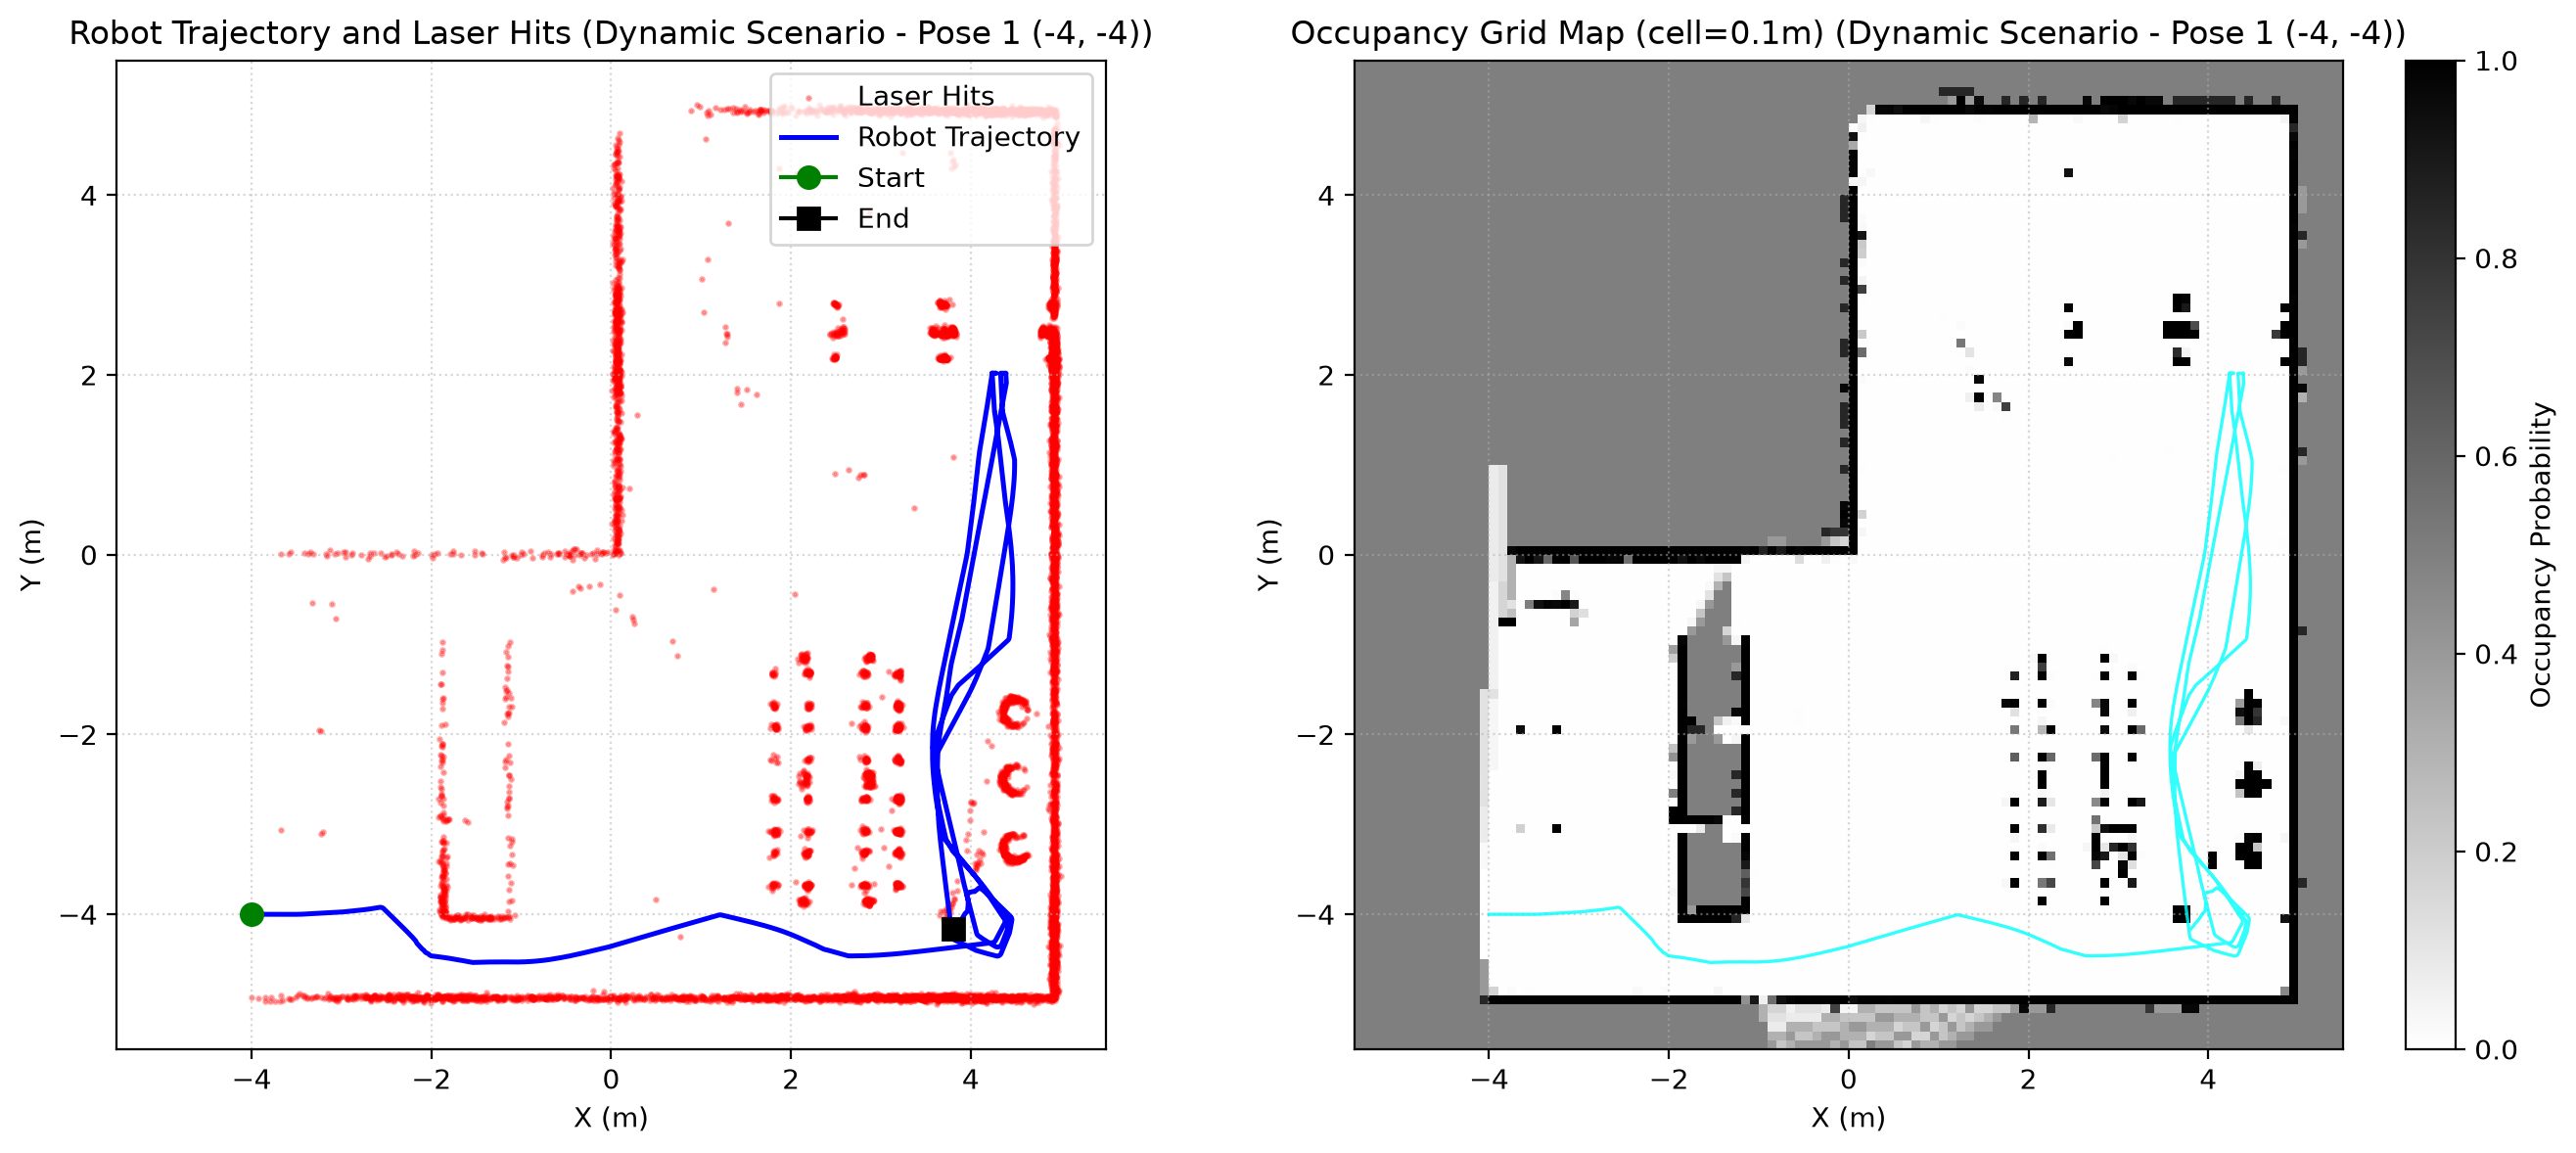
\includegraphics[width=\textwidth]{results/exp4_dynamic_pos1_overview.png}
    \caption{Cenário Dinâmico — Posição Inicial 1 $(-4{,}0, -4{,}0)$\,m: Trajetória com pedestre móvel (esq.) e Occupancy Grid gerado (dir.).}
    \label{fig:dyn_pos1}
\end{figure}

\begin{figure}[htbp]
    \centering
    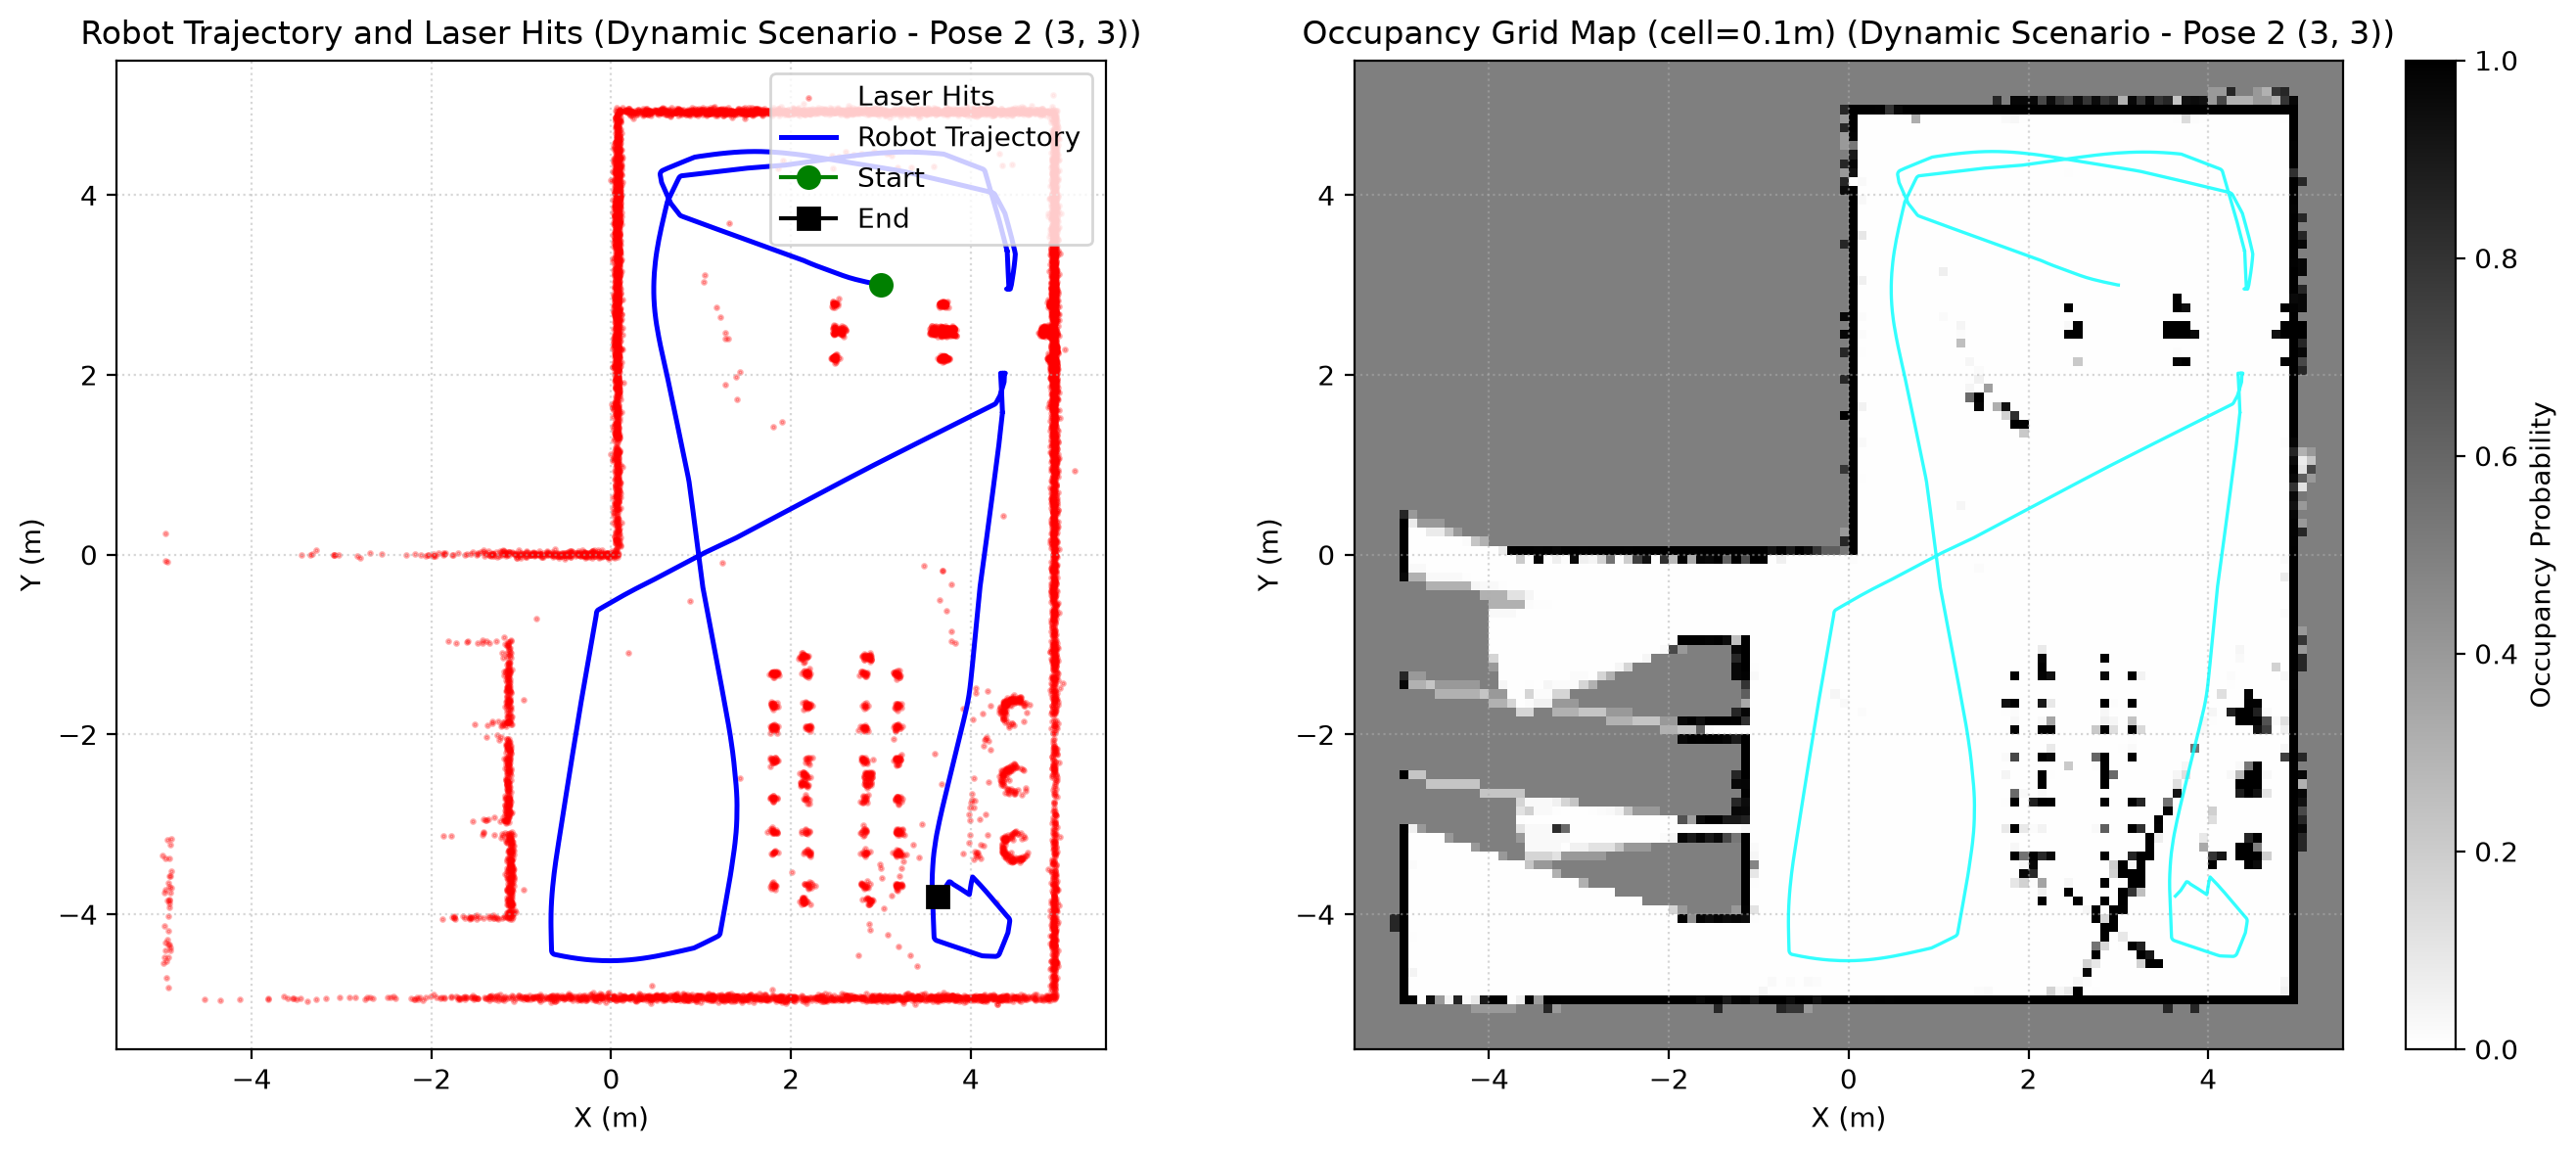
\includegraphics[width=\textwidth]{results/exp5_dynamic_pos2_overview.png}
    \caption{Cenário Dinâmico — Posição Inicial 2 $(+3{,}0, +3{,}0)$\,m: Trajetória com pedestre móvel (esq.) e Occupancy Grid gerado (dir.).}
    \label{fig:dyn_pos2}
\end{figure}

\subsubsection{Análise do Impacto de Obstáculos Dinâmicos}
O modelo de Occupancy Grid clássico baseia-se na suposição de que o ambiente é puramente estático ($p(m_i | z_t) = p(m_i)$). A presença do humano em movimento produz dois efeitos notáveis:
\begin{enumerate}
    \item \textbf{Rastros Transitórios de Ocupação:} Nos pontos onde o humano permaneceu temporariamente durante varreduras do laser, as células correspondentes receberam incrementos positivos $\Delta l_{occ}$, gerando manchas acinzentadas ao longo de sua trajetória (visíveis, por exemplo, na diagonal inferior direita da Figura \ref{fig:dyn_pos2}).
    \item \textbf{Efeito de Limpeza por Observações Posteriores:} À medida que o humano se desloca e o robô realiza novas varreduras sobre a região agora desobstruída, os feixes propagam-se livremente e aplicam repetidas deduções $\Delta l_{free}$. Dessa forma, células que antes continham rastros do pedestre têm sua probabilidade de ocupação atenuada de volta para o nível livre, demonstrando a capacidade adaptativa inerente à formulação de log-odds saturado.
\end{enumerate}

\subsection{Experimento 4: Estudo de Sensibilidade ao Ruído Sensorial}
Para avaliar a robustez do mapeamento probabilístico, introduziu-se ruído gaussiano sintético $\mathcal{N}(0, \sigma_r^2)$ na distância medida e $\mathcal{N}(0, \sigma_\theta^2)$ no ângulo dos feixes. Avaliaram-se três regimes de perturbação (Figura \ref{fig:noise_comparison}):
\begin{itemize}
    \item \textbf{Baixo Ruído:} $\sigma_r = 0{,}01$\,m ($1$\,cm), $\sigma_\theta = 0{,}002$\,rad ($\approx 0{,}1^\circ$).
    \item \textbf{Médio Ruído:} $\sigma_r = 0{,}05$\,m ($5$\,cm), $\sigma_\theta = 0{,}010$\,rad ($\approx 0{,}6^\circ$).
    \item \textbf{Alto Ruído:} $\sigma_r = 0{,}15$\,m ($15$\,cm), $\sigma_\theta = 0{,}030$\,rad ($\approx 1{,}7^\circ$).
\end{itemize}

\begin{figure}[htbp]
    \centering
    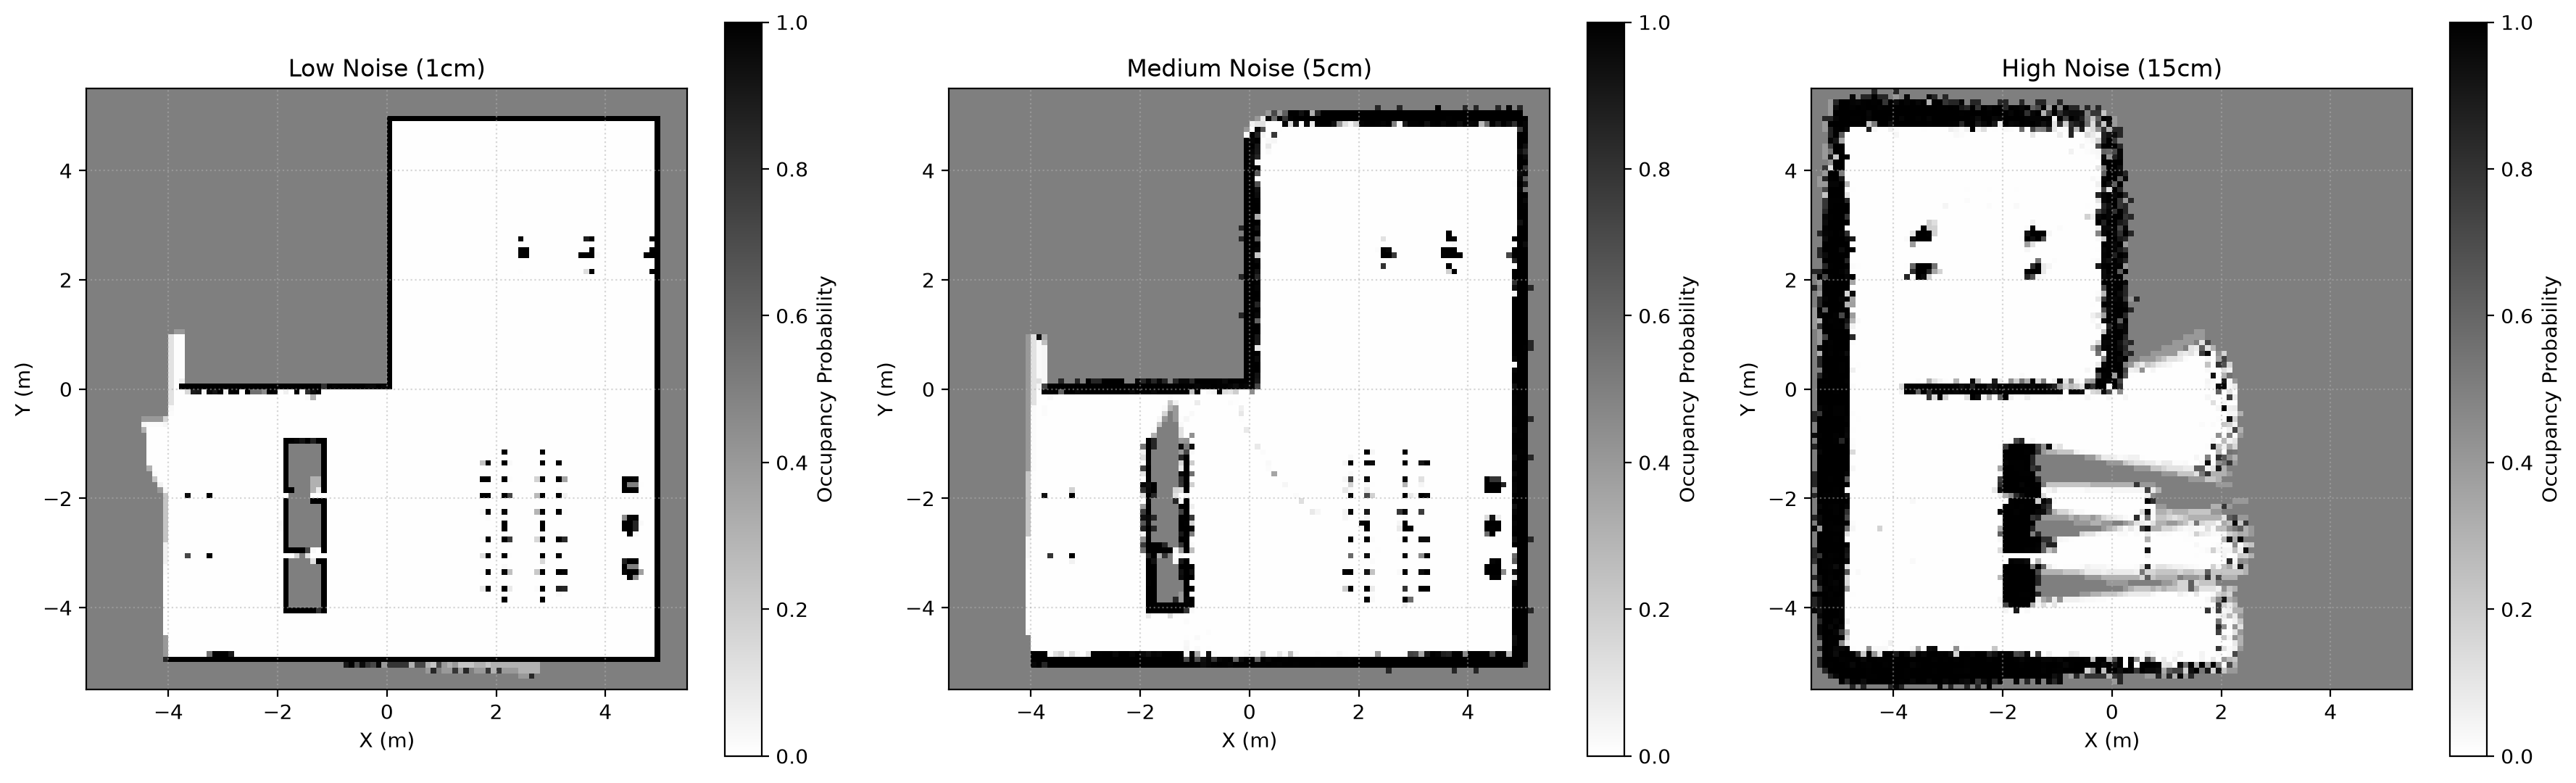
\includegraphics[width=\textwidth]{results/exp_noise_comparison.png}
    \caption{Estudo de sensibilidade ao ruído do sensor laser: (a) Baixo ruído ($1$\,cm); (b) Médio ruído ($5$\,cm); (c) Alto ruído ($15$\,cm).}
    \label{fig:noise_comparison}
\end{figure}

\subsubsection{Discussão da Robustez Probabilística}
Sob ruído moderado ($5$\,cm), a espessura aparente das paredes sofre mínima variação e a geometria geral permanece perfeitamente nítida, demonstrando que a integração recursiva do filtro bayesiano atua como um filtro passa-baixas eficiente que atenua ruídos de média zero. Sob ruído extremo ($15$\,cm), verifica-se espessamento das fronteiras e dispersão nas quinas dos móveis, evidenciando o limite a partir do qual a incerteza de medição supera a resolução da célula.

\section{Conclusões e Principais Dificuldades}

O projeto foi concluído com pleno êxito, satisfazendo integralmente todas as exigências especificadas:
\begin{itemize}
    \item A implementação modular em Python com o ambiente UV resultou em código limpo, simples, legível e livre de complexidades desnecessárias.
    \item O algoritmo de Occupancy Grid em log-odds provou ser rápido, estável e computacionalmente leve, viabilizando geração de mapas de alta qualidade em tempo real.
    \item O navegador reativo garantiu cobertura abrangente do salão sem bloqueios nem colisões.
    \item As análises comparativas de resolução, posições iniciais, dinâmica e ruído sensorial forneceram compreensão aprofundada das propriedades e limitações práticas das grades de ocupação.
\end{itemize}

\subsection{Dificuldades Encontradas e Soluções}
\begin{itemize}
    \item \textbf{Extração de Sinais Binários no CoppeliaSim 4.10:} O script nativo do \texttt{fastHokuyo} compacta os 684 alcances e ângulos com \texttt{sim.packFloatTable}. No CoppeliaSim 4.10, dados empacotados como buffer binário devem ser recuperados via \texttt{sim.getBufferSignal} em vez de \texttt{sim.getStringSignal}. O uso de \texttt{getBufferSignal} garantiu transferência direta de 2736 bytes em microssegundos.
    \item \textbf{Aceleração de Renderização em Container Docker:} A configuração inicial do container na máquina utilizava renderização integrada Mesa sobre a GPU AMD Rembrandt, apresentando baixo desempenho no XWayland. A resolução consistiu na integração do \textit{NVIDIA Container Toolkit} com CDI (\textit{Container Device Interface}), habilitando passagem nativa dos nós de dispositivo e bibliotecas proprietárias para a GPU dedicada NVIDIA GeForce RTX 3050 Laptop, acelerando a execução.
\end{itemize}

\begin{thebibliography}{99}
\bibitem{moravec1985}
H. P. Moravec and A. E. Elfes, ``High resolution maps from wide angle sonar,'' in \textit{Proc. IEEE International Conference on Robotics and Automation (ICRA)}, 1985, pp. 116--121.

\bibitem{thrun2005}
S. Thrun, W. Burgard, and D. Fox, \textit{Probabilistic Robotics}. Cambridge, MA: MIT Press, 2005.

\bibitem{kobuki}
Yujin Robot, ``Kobuki Parameters and Documentation,'' [Online]. Disponível em: \url{https://yujinrobot.github.io/kobuki/enAppendixKobukiParameters.html}.

\bibitem{coppelia}
Coppelia Robotics, ``CoppeliaSim ZMQ Remote API Documentation,'' [Online]. Disponível em: \url{https://manual.coppeliarobotics.com/}.
\end{thebibliography}

\end{document}
